\subsubsection{Sequential switching between Tent and Logistic maps (SWITCH)} \label{sssec:switch}

SWITCH may be expressed as:

\textcolor{red}{ESTA ECUACIÓN HAY QUE REVISARLA, CREO QUE CON PONER QUE n ES UN NÚMERO PAR INCLUÍDO EL CERO ES SUFICIENTE}
\[ \left\{ \begin{array}{ccc}\label{eq:seq}
	x_{n+1}&~=&~ \left\{ \begin{array}{ll}
		2~{x_n}  \textrm{if $0\leq x_n\leq 1/2$}\\
		2~(1-{x_n})  \textrm{if $1/2<x_n\leq 1$} 
	\end{array} \right 
	\\ x_{n+2}&~=&~ 4~x_{n+1}~(1-x_{n+1}) \\
\end{array}\right. \] 
with $x_n\in\mathcal{R}$ and $n$ an even number.

Results with sequential switching are shown in Figs. \ref{fig:SWITCH_QuantiB} (a) to (f).
The floating point entropy value is $H_{val}=0.9722$, a marginal increment value to that obtained for LOG. 
For fractinal numbers this value is reached for $B=24$, but it is stable from $B=28$.
Regarding ordering patterns the number of MP decreases to $586$, a value lower than the one obtained for LOG.
It means the entropy $H_{BP}$ may increase up to $ln(134)/ln(720)\simeq 0.74$.
$BP$ and $BPW$ quantifiers reachs their maximum of $H_{BP}=0.6546$ and $H_{BPW}=0.6313$ at $B=16$, but they stabilishes at $B=24$.
Complexities are lower than LOG, $C_{BP}=0.4580$ and $C_{BPW}=0.4578$, these values are reached for $B \geq 15$ but is stable from $B \geq 23$.
Compared with LOG, statistical proerties are better and they are reached with a less amount of bits, for $B \geq 24$ this map reachs optimal characteristics.

We can see some points with anomalies from $B \geq 49$ due to same problem of LOG map, an multiplication needs double of precision to be done.
Furthermore, we encountred one initial condition in fixed point with an anomalous behaviour.

\begin{figure}
	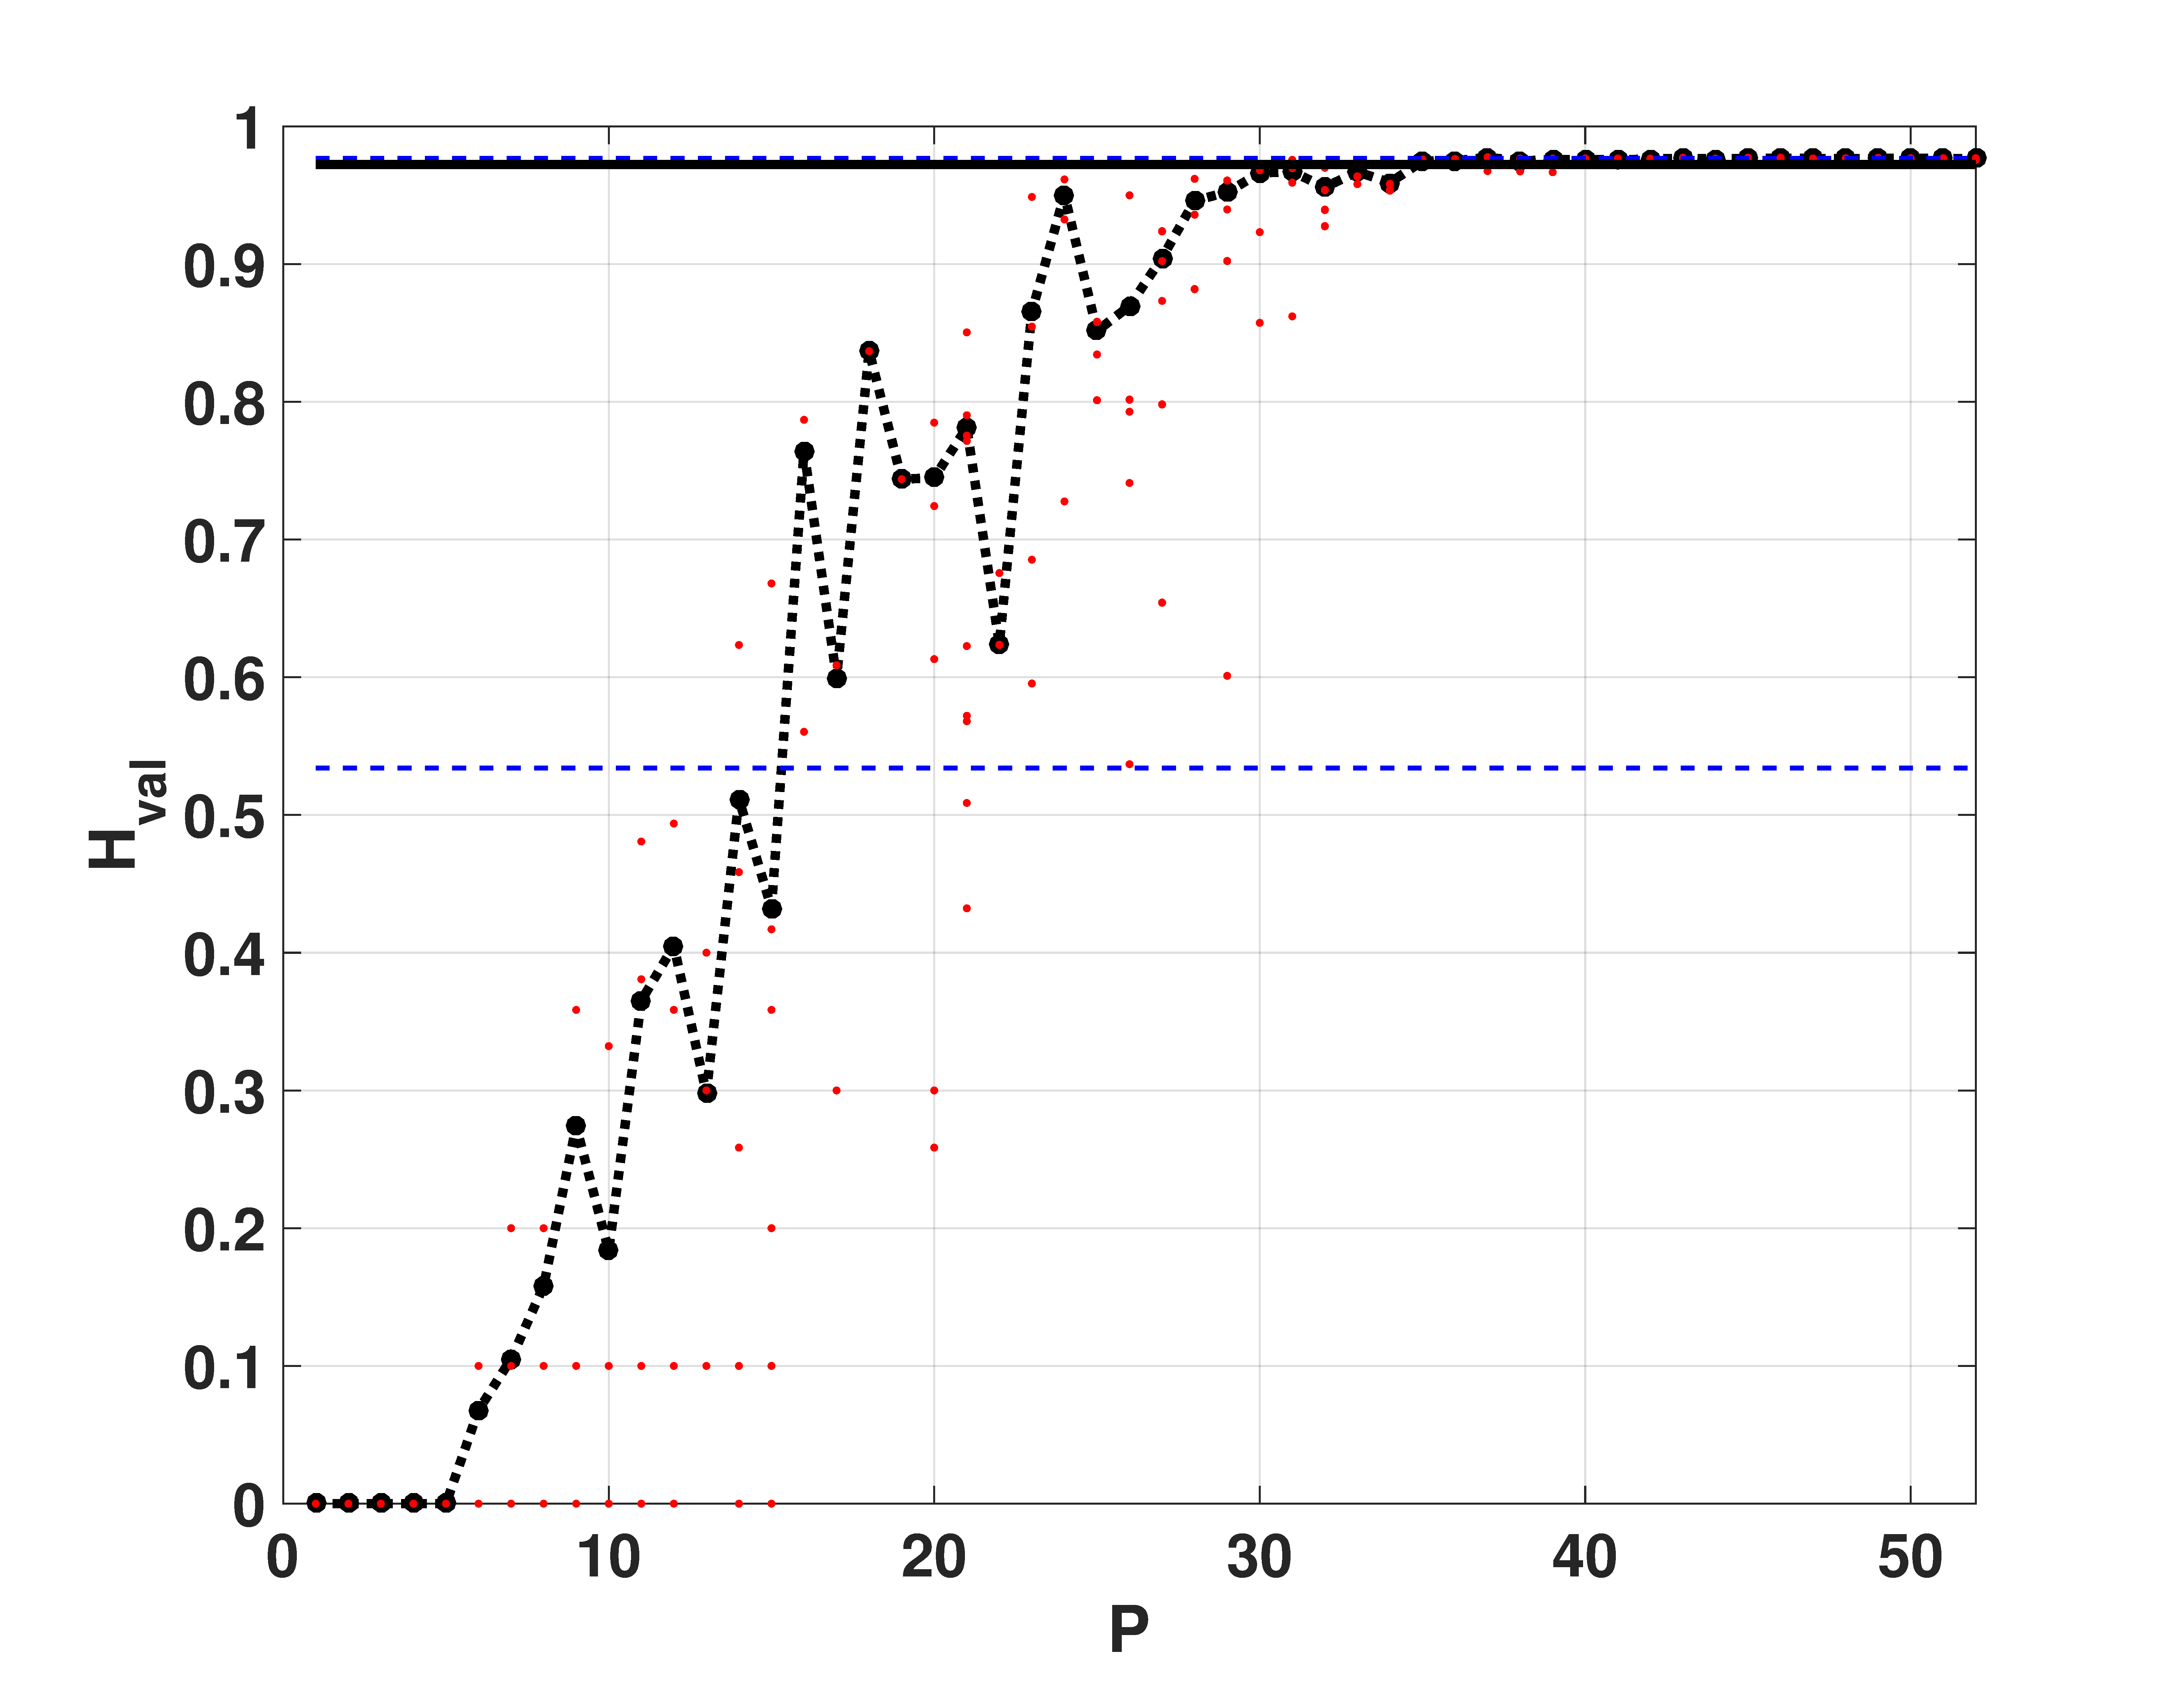
\includegraphics[width=.49\textwidth]{Hval_Switch}
	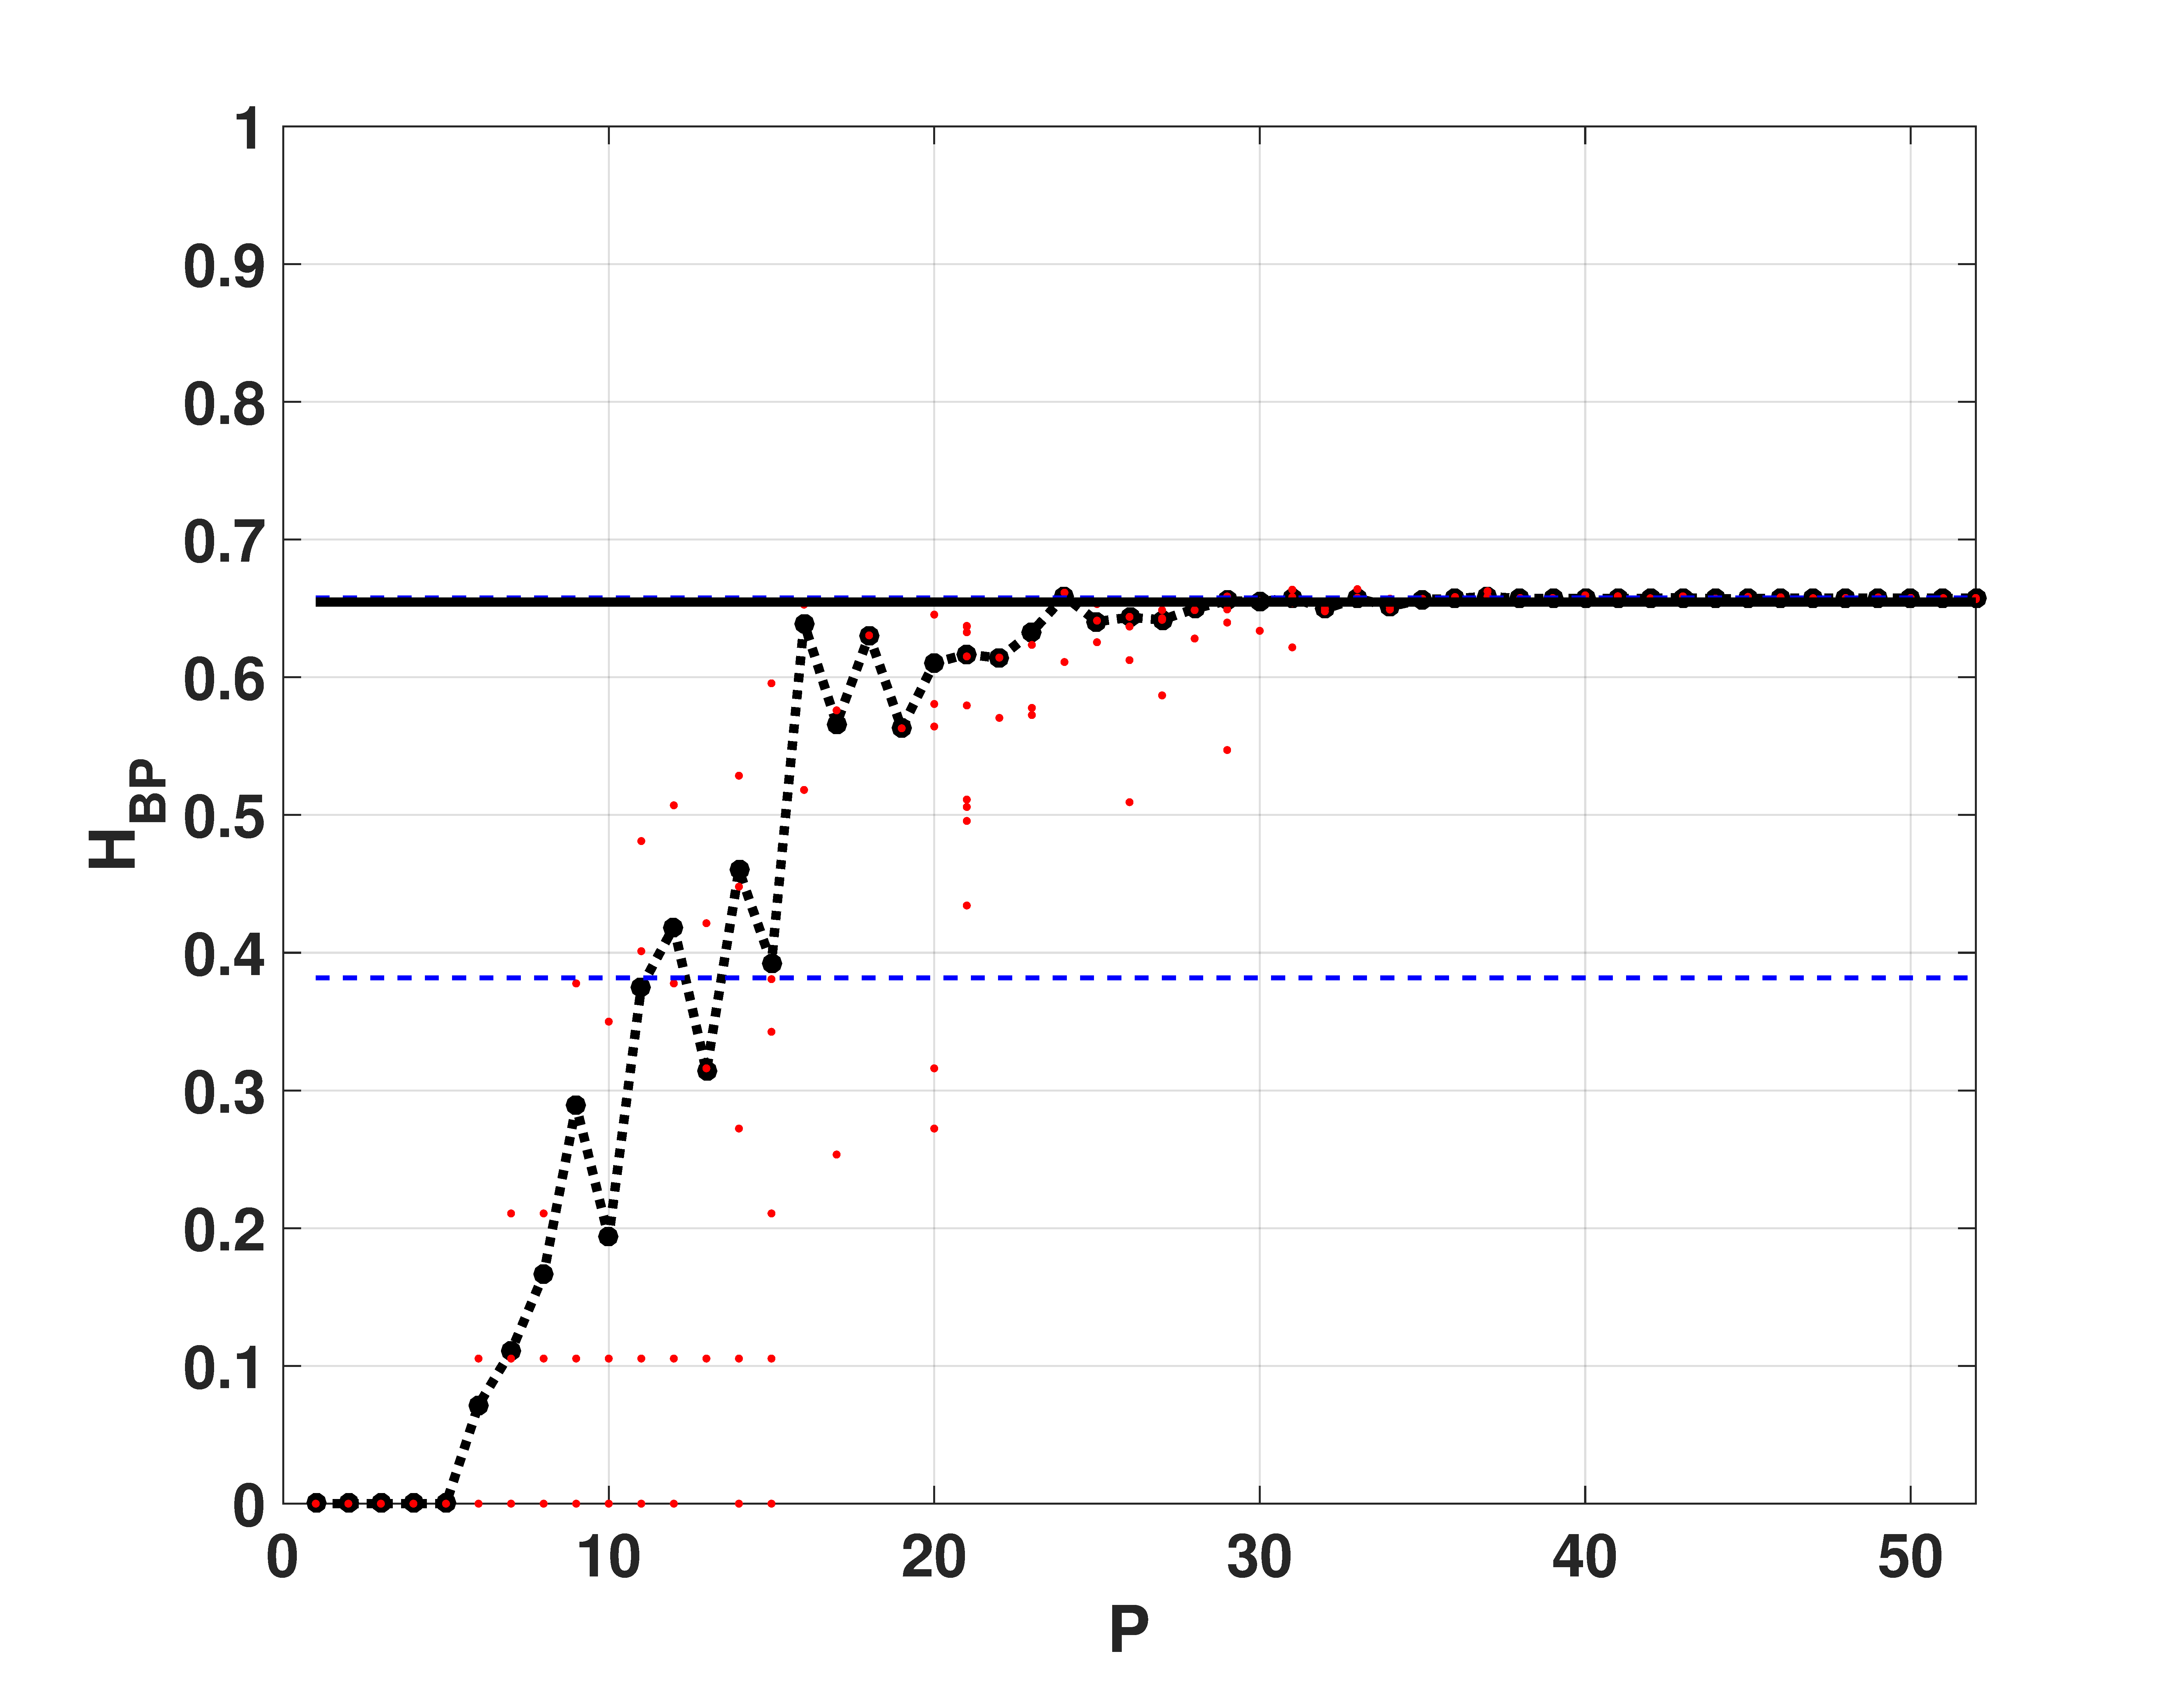
\includegraphics[width=.49\textwidth]{Hbp_Switch}
	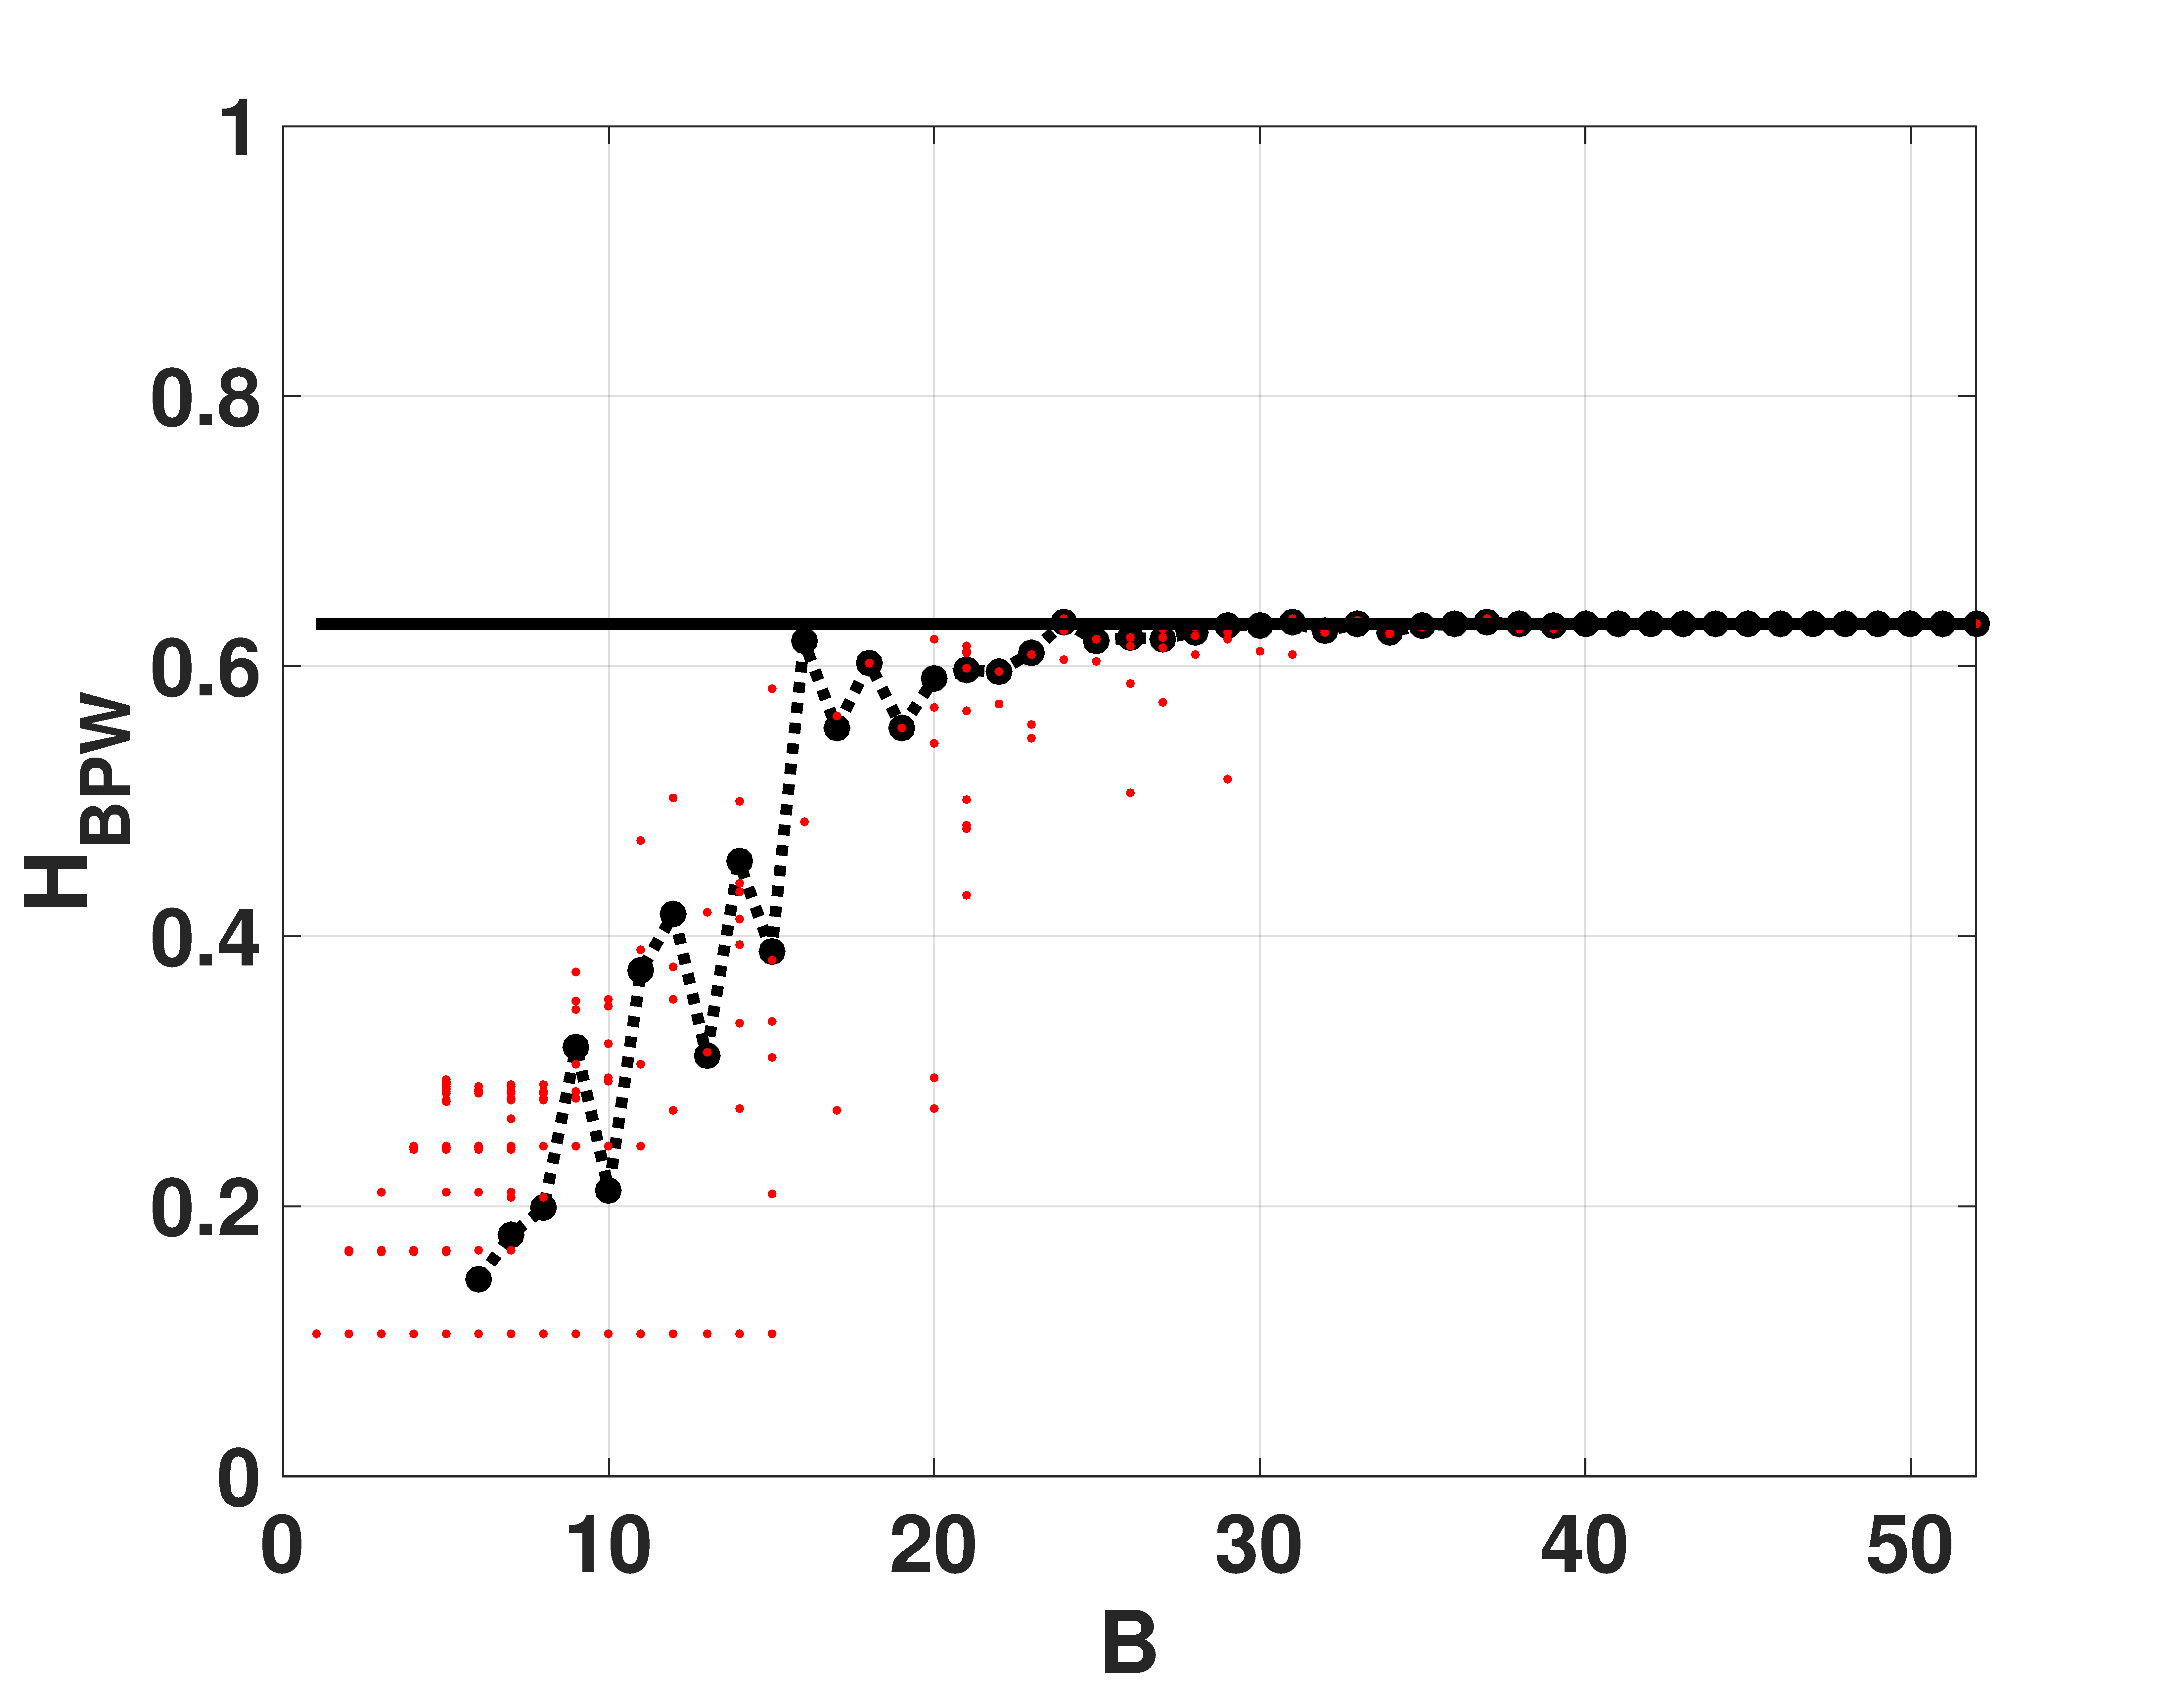
\includegraphics[width=.49\textwidth]{Hbpw_Switch}
	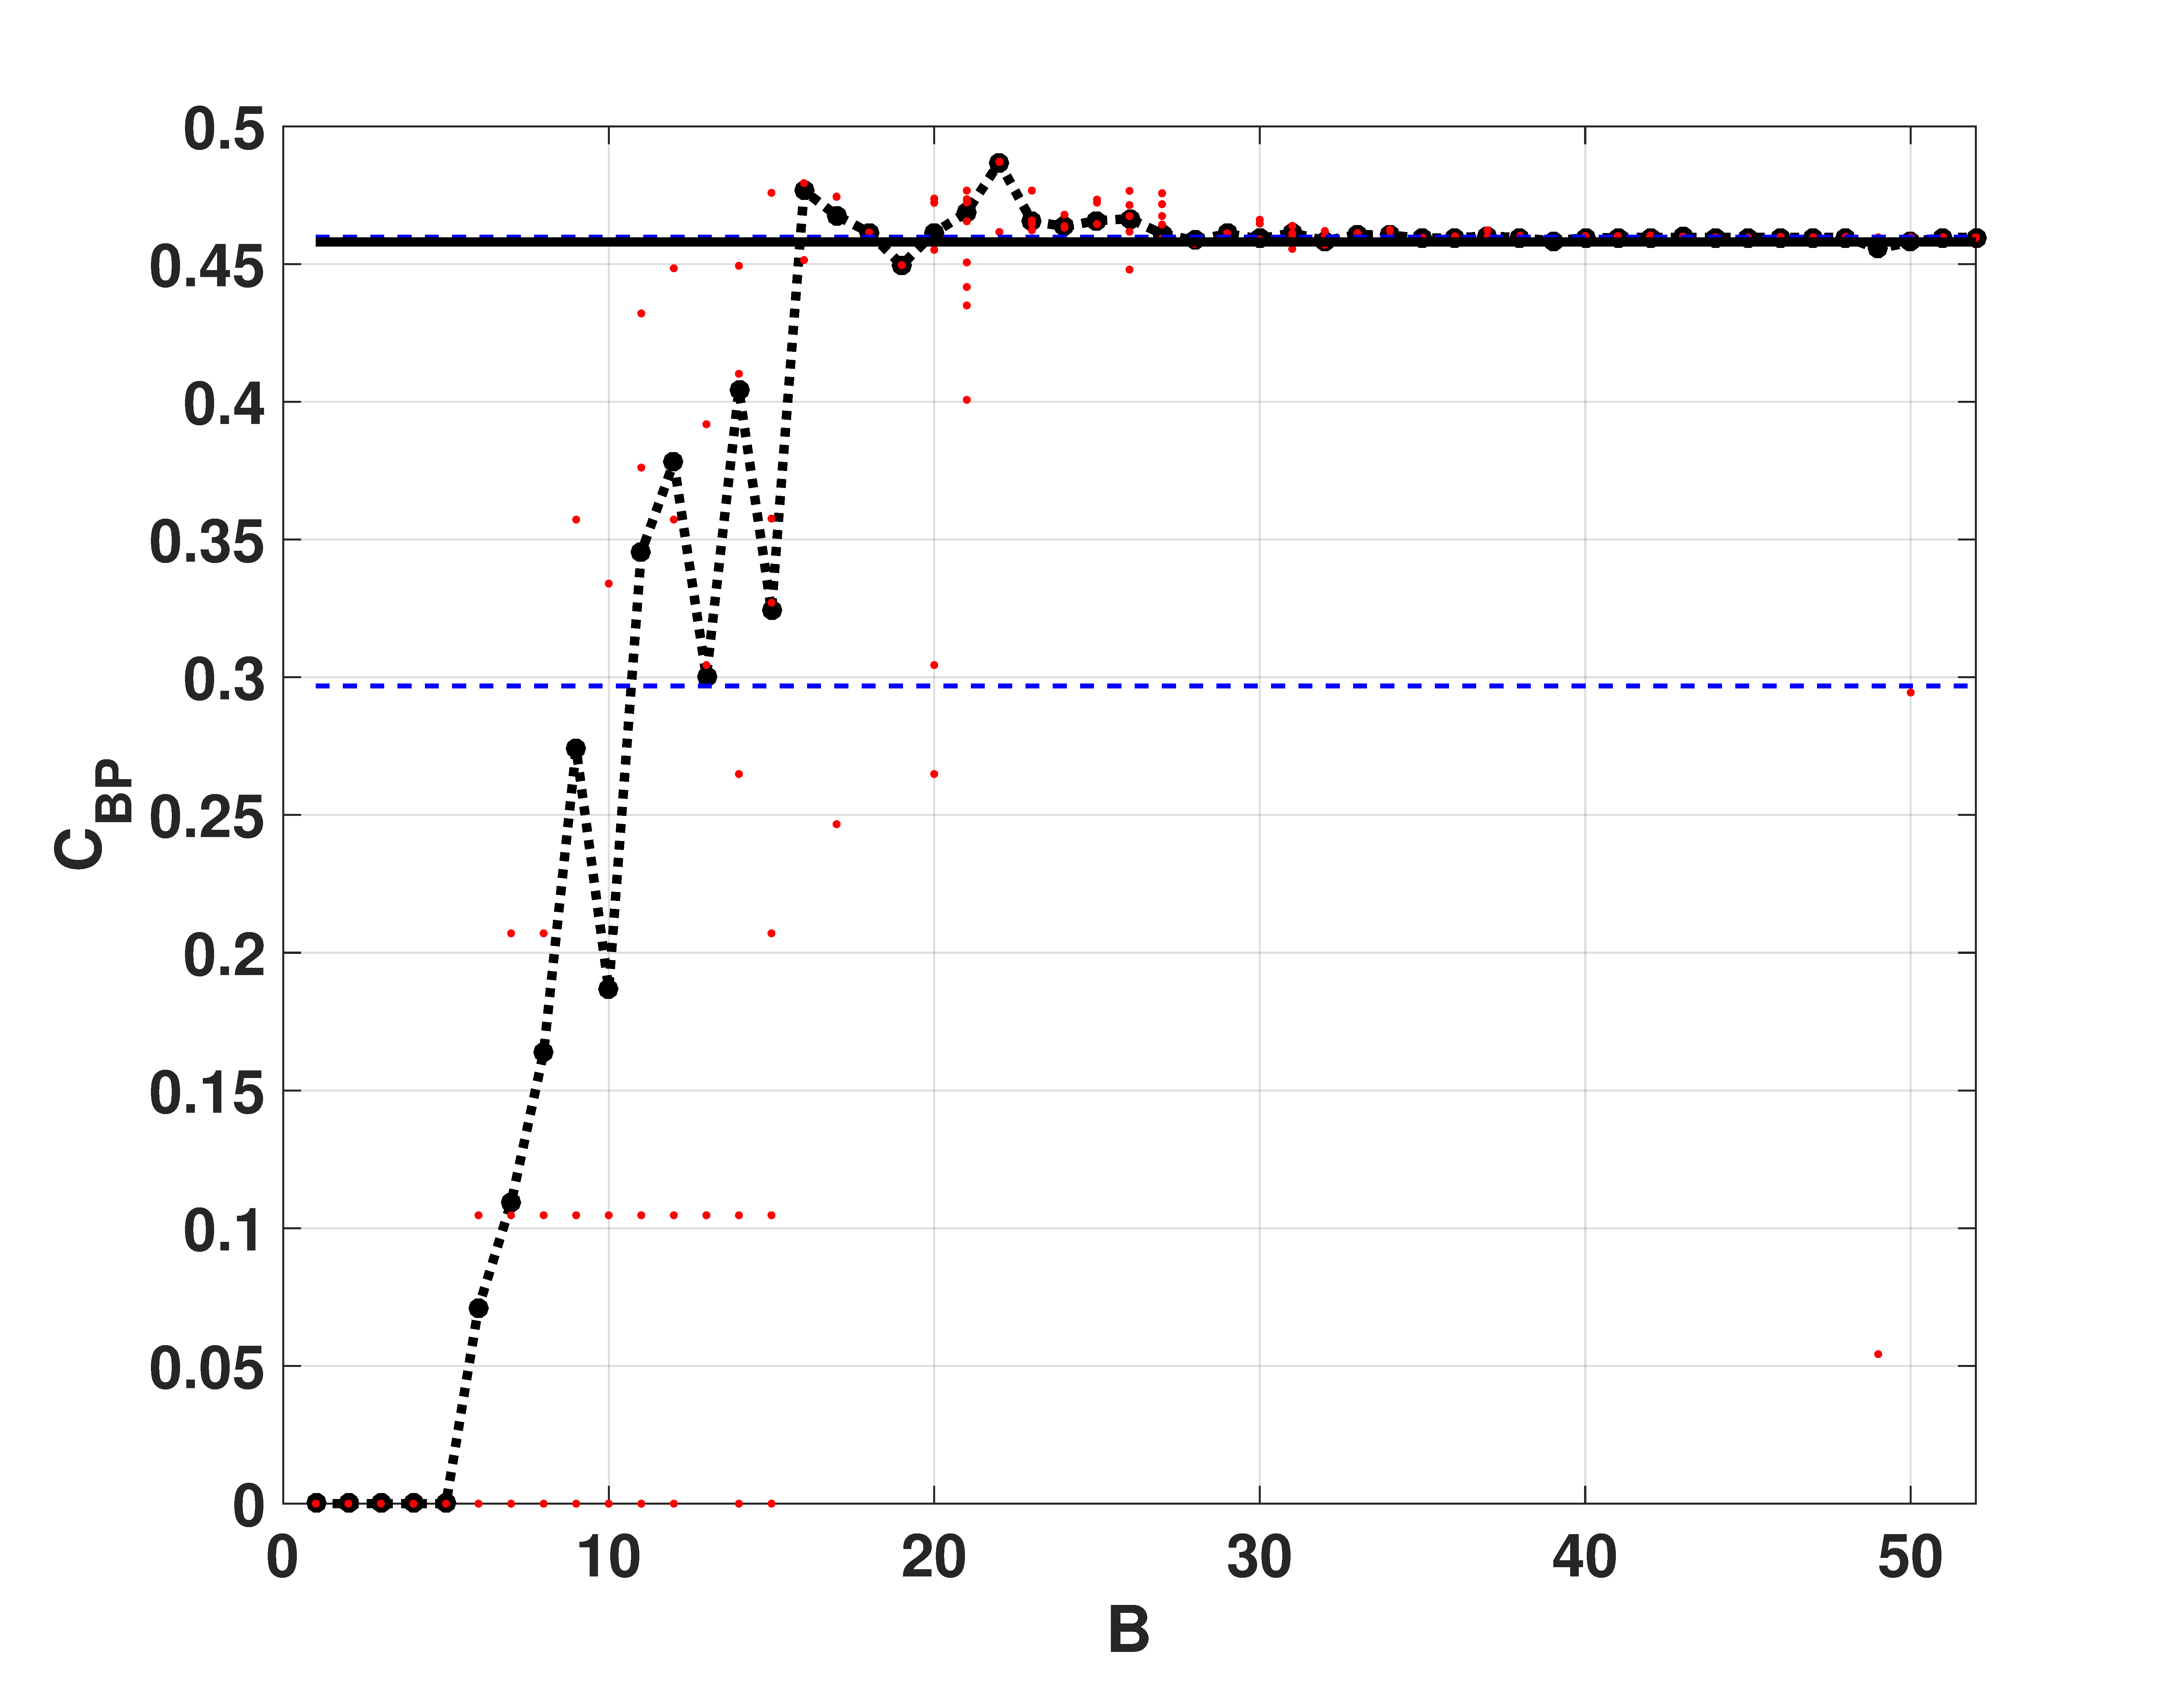
\includegraphics[width=.49\textwidth]{Cbp_Switch}
	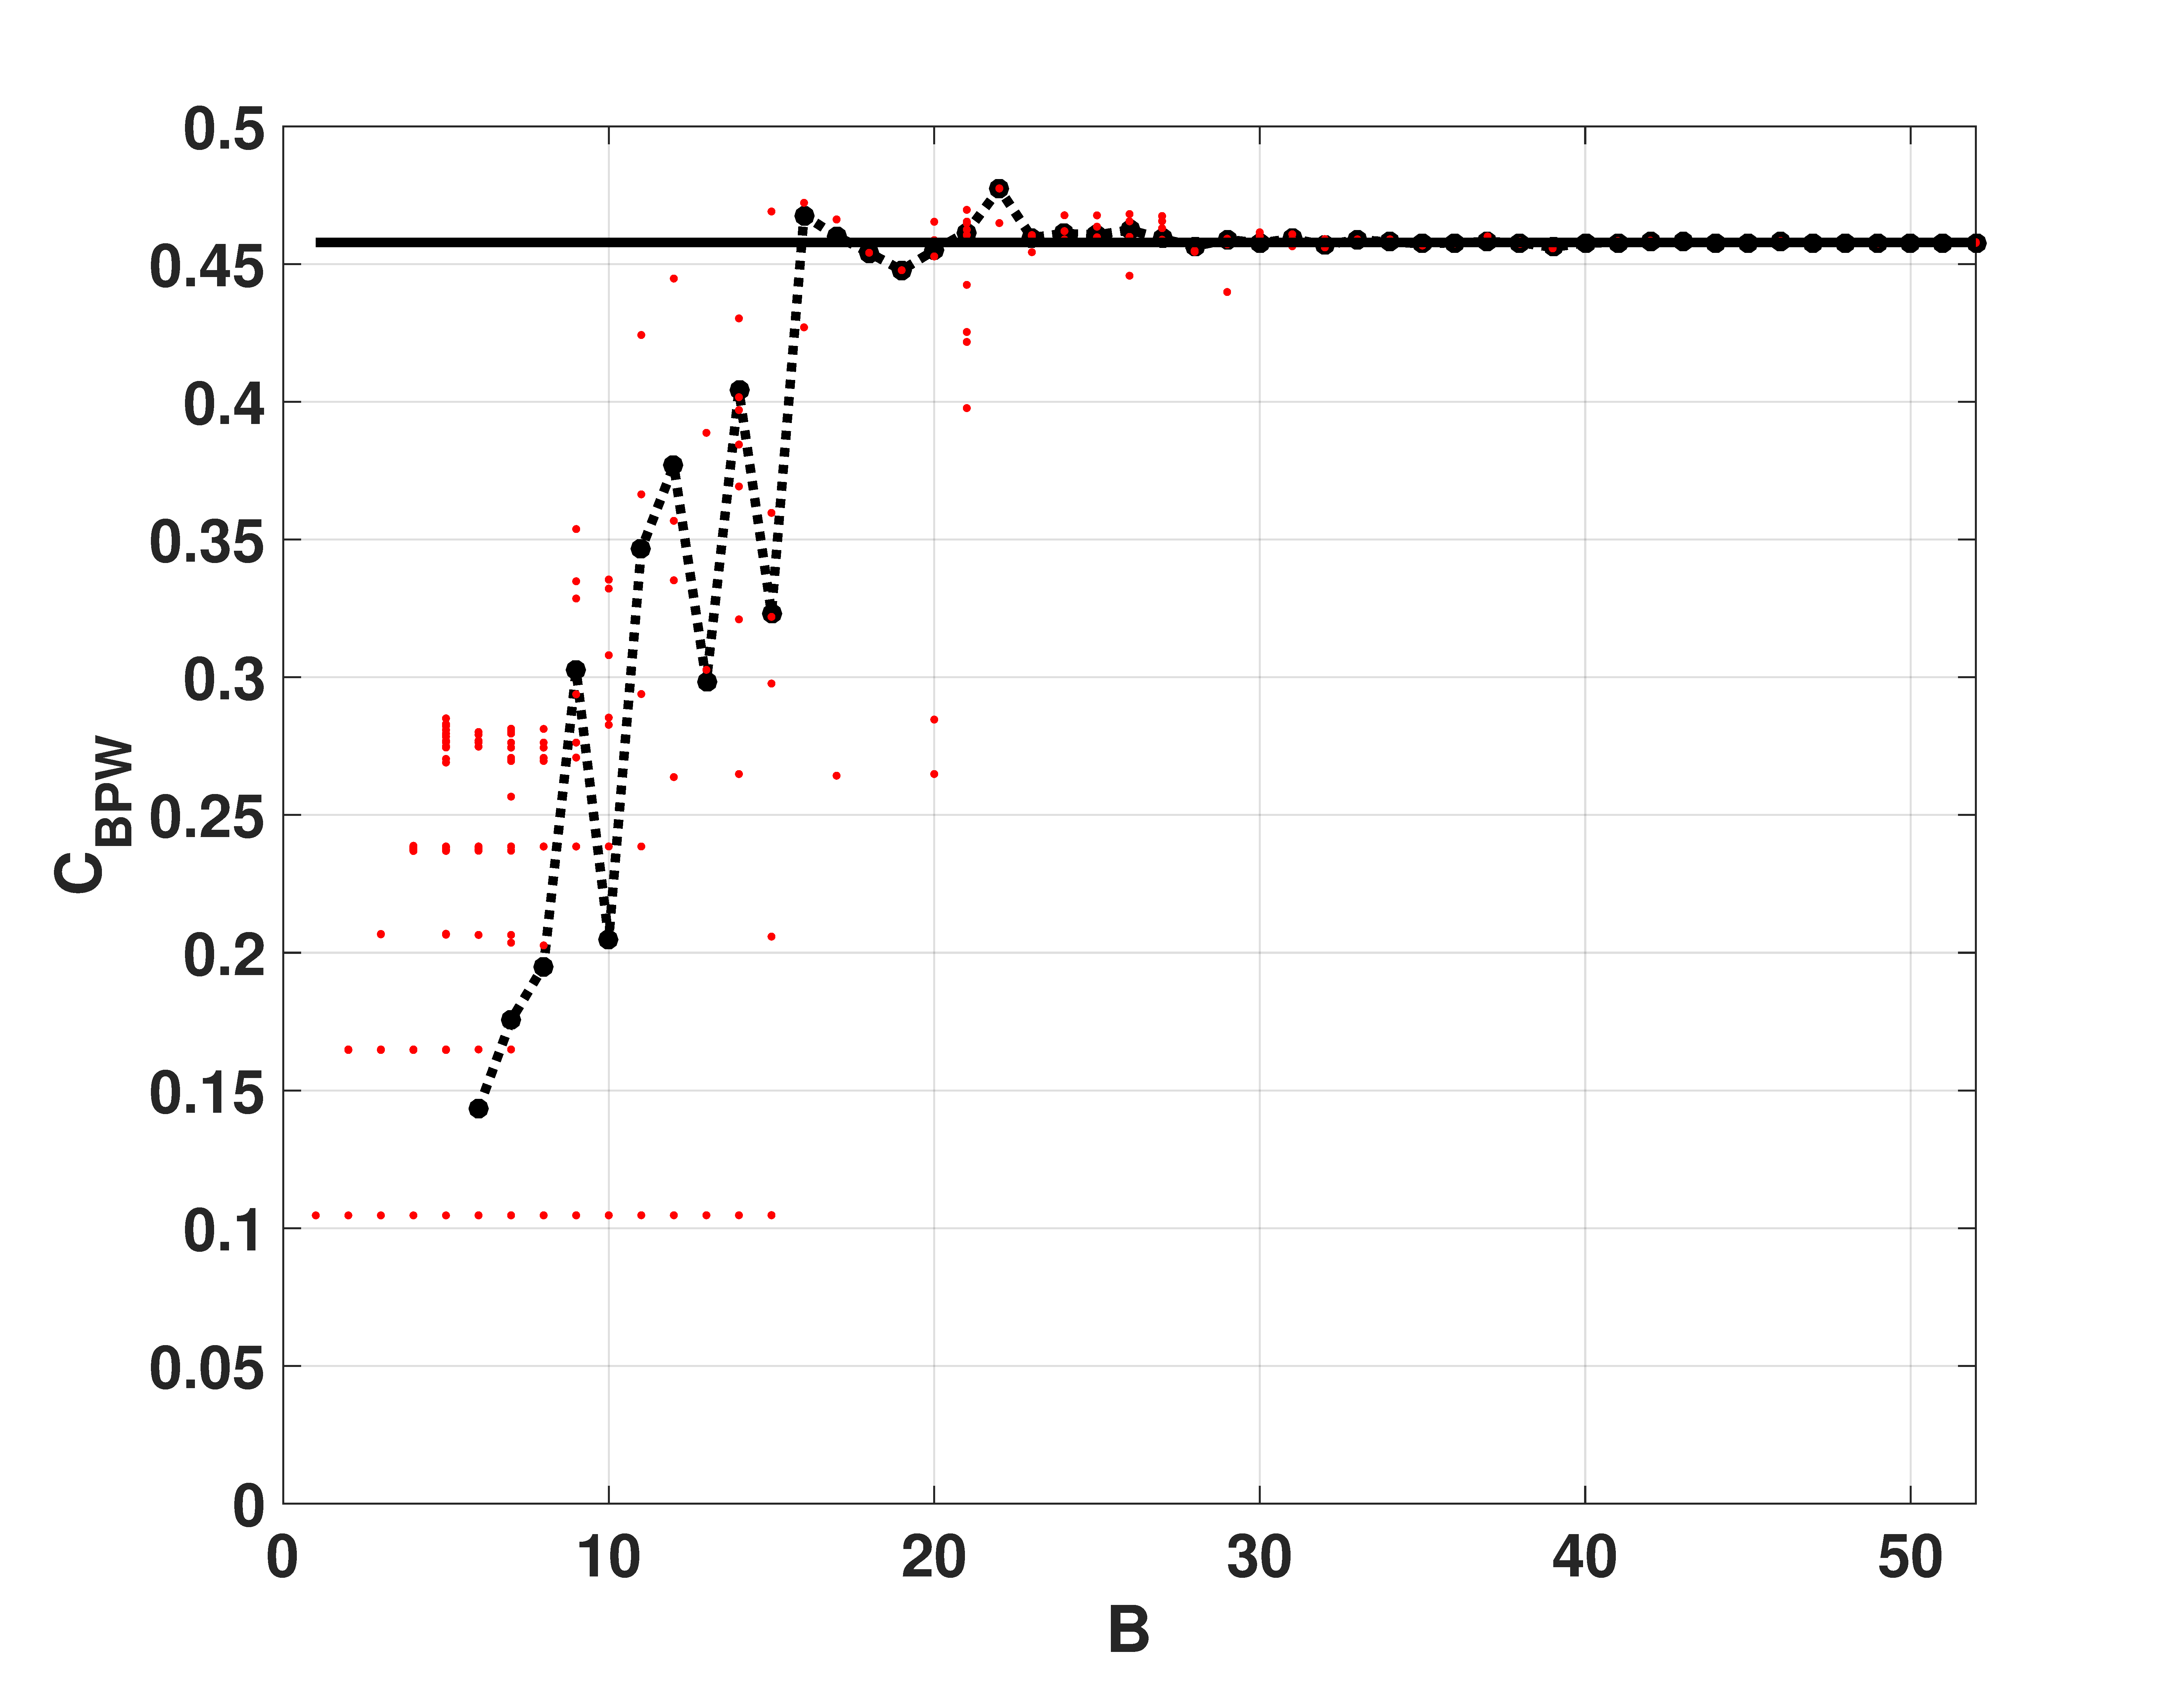
\includegraphics[width=.49\textwidth]{Cbpw_Switch}
	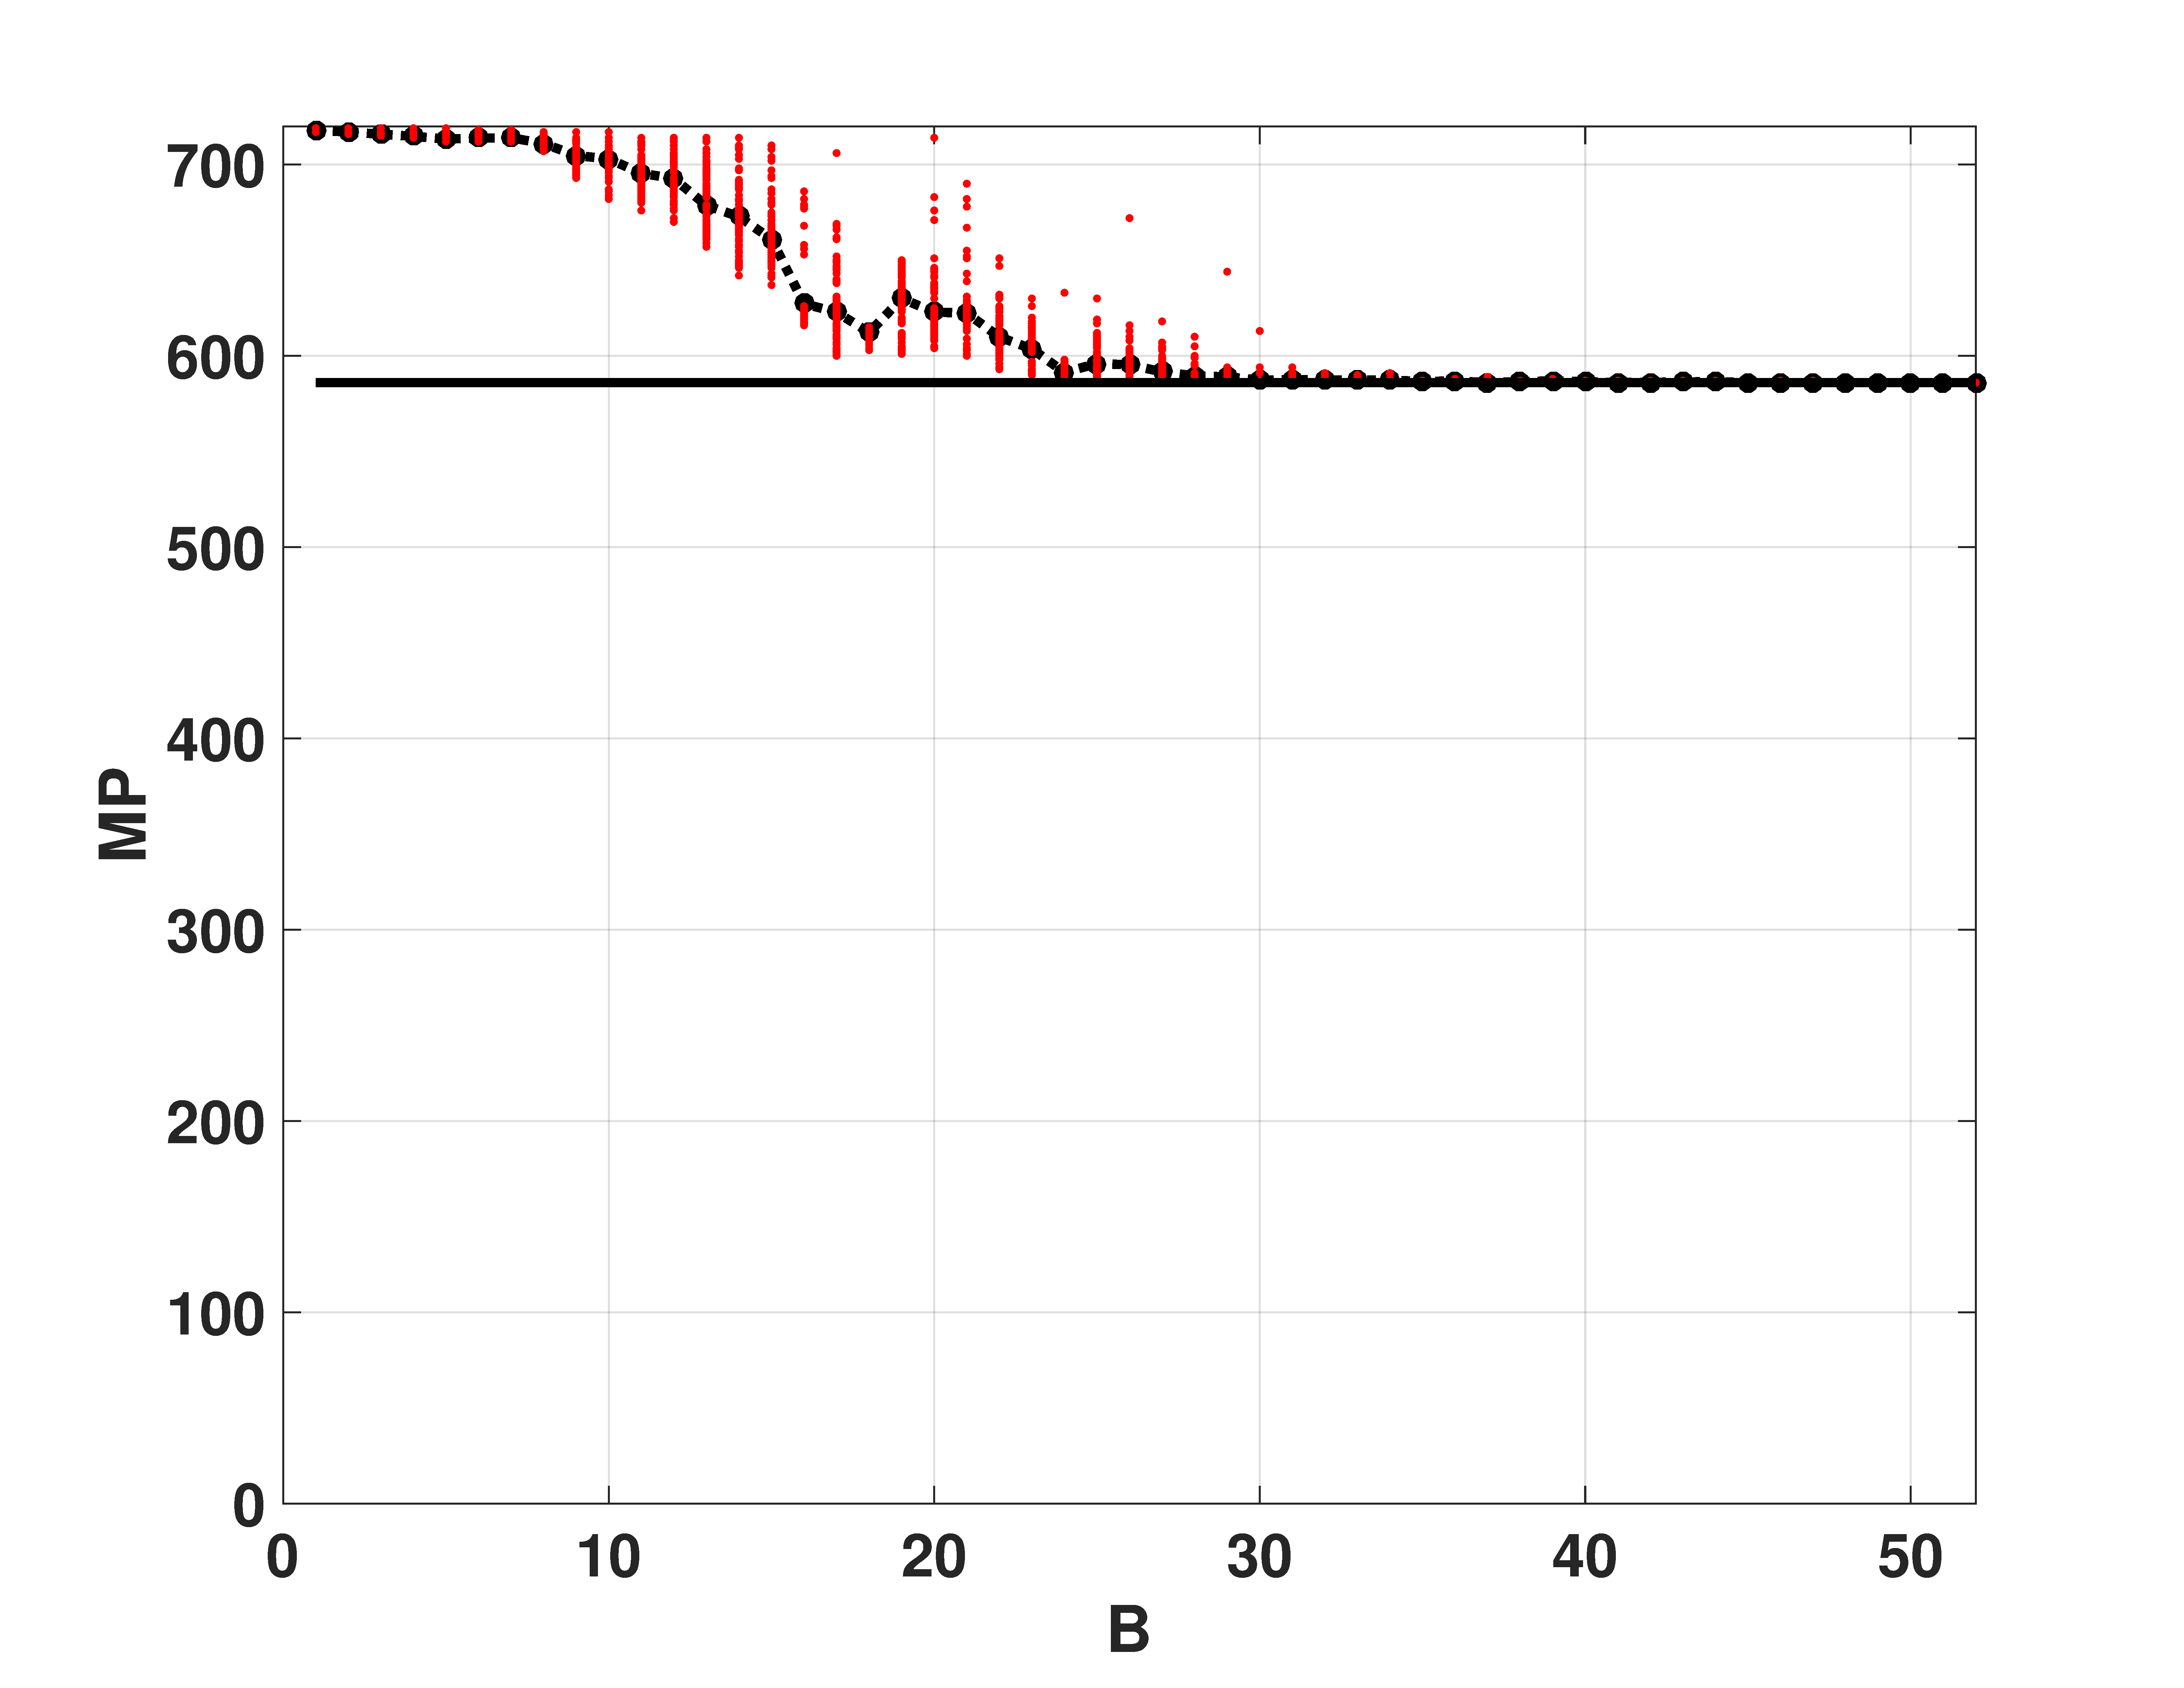
\includegraphics[width=.49\textwidth]{MP_Switch}
	\caption{Statistical properties of the SWITCH map using binary representation: (a) $H_{val}$ vs $B$ (b) $H_{BP}$ vs $B$ (c) $C_{BP}$ vs $B$ (d) Number of missing ordering patterns $MP$ vs $B$.}
	\label{fig:SWITCH_QuantiB}
\end{figure}

Double entropy plane $H_{val}$ vs $H_{BP}$ is showed in Fig. \ref{fig:SWITCH_HH}.
The point reached in this plane for SWITCH map is similar than reached for LOG map, there is a small difference on vertical axis.
It means that mixing is beter for SWITCH.

\textcolor{red}{TENDRÍA QUE SACAR MAS CONCLUSIONES DE LOS PLANOS TENDRÍA QUE VERLAS EN LAS SERIES DE DATOS, ESPECIALMENTE EL PUNTO ESE QUE DA CORRIDO}

\begin{figure}
	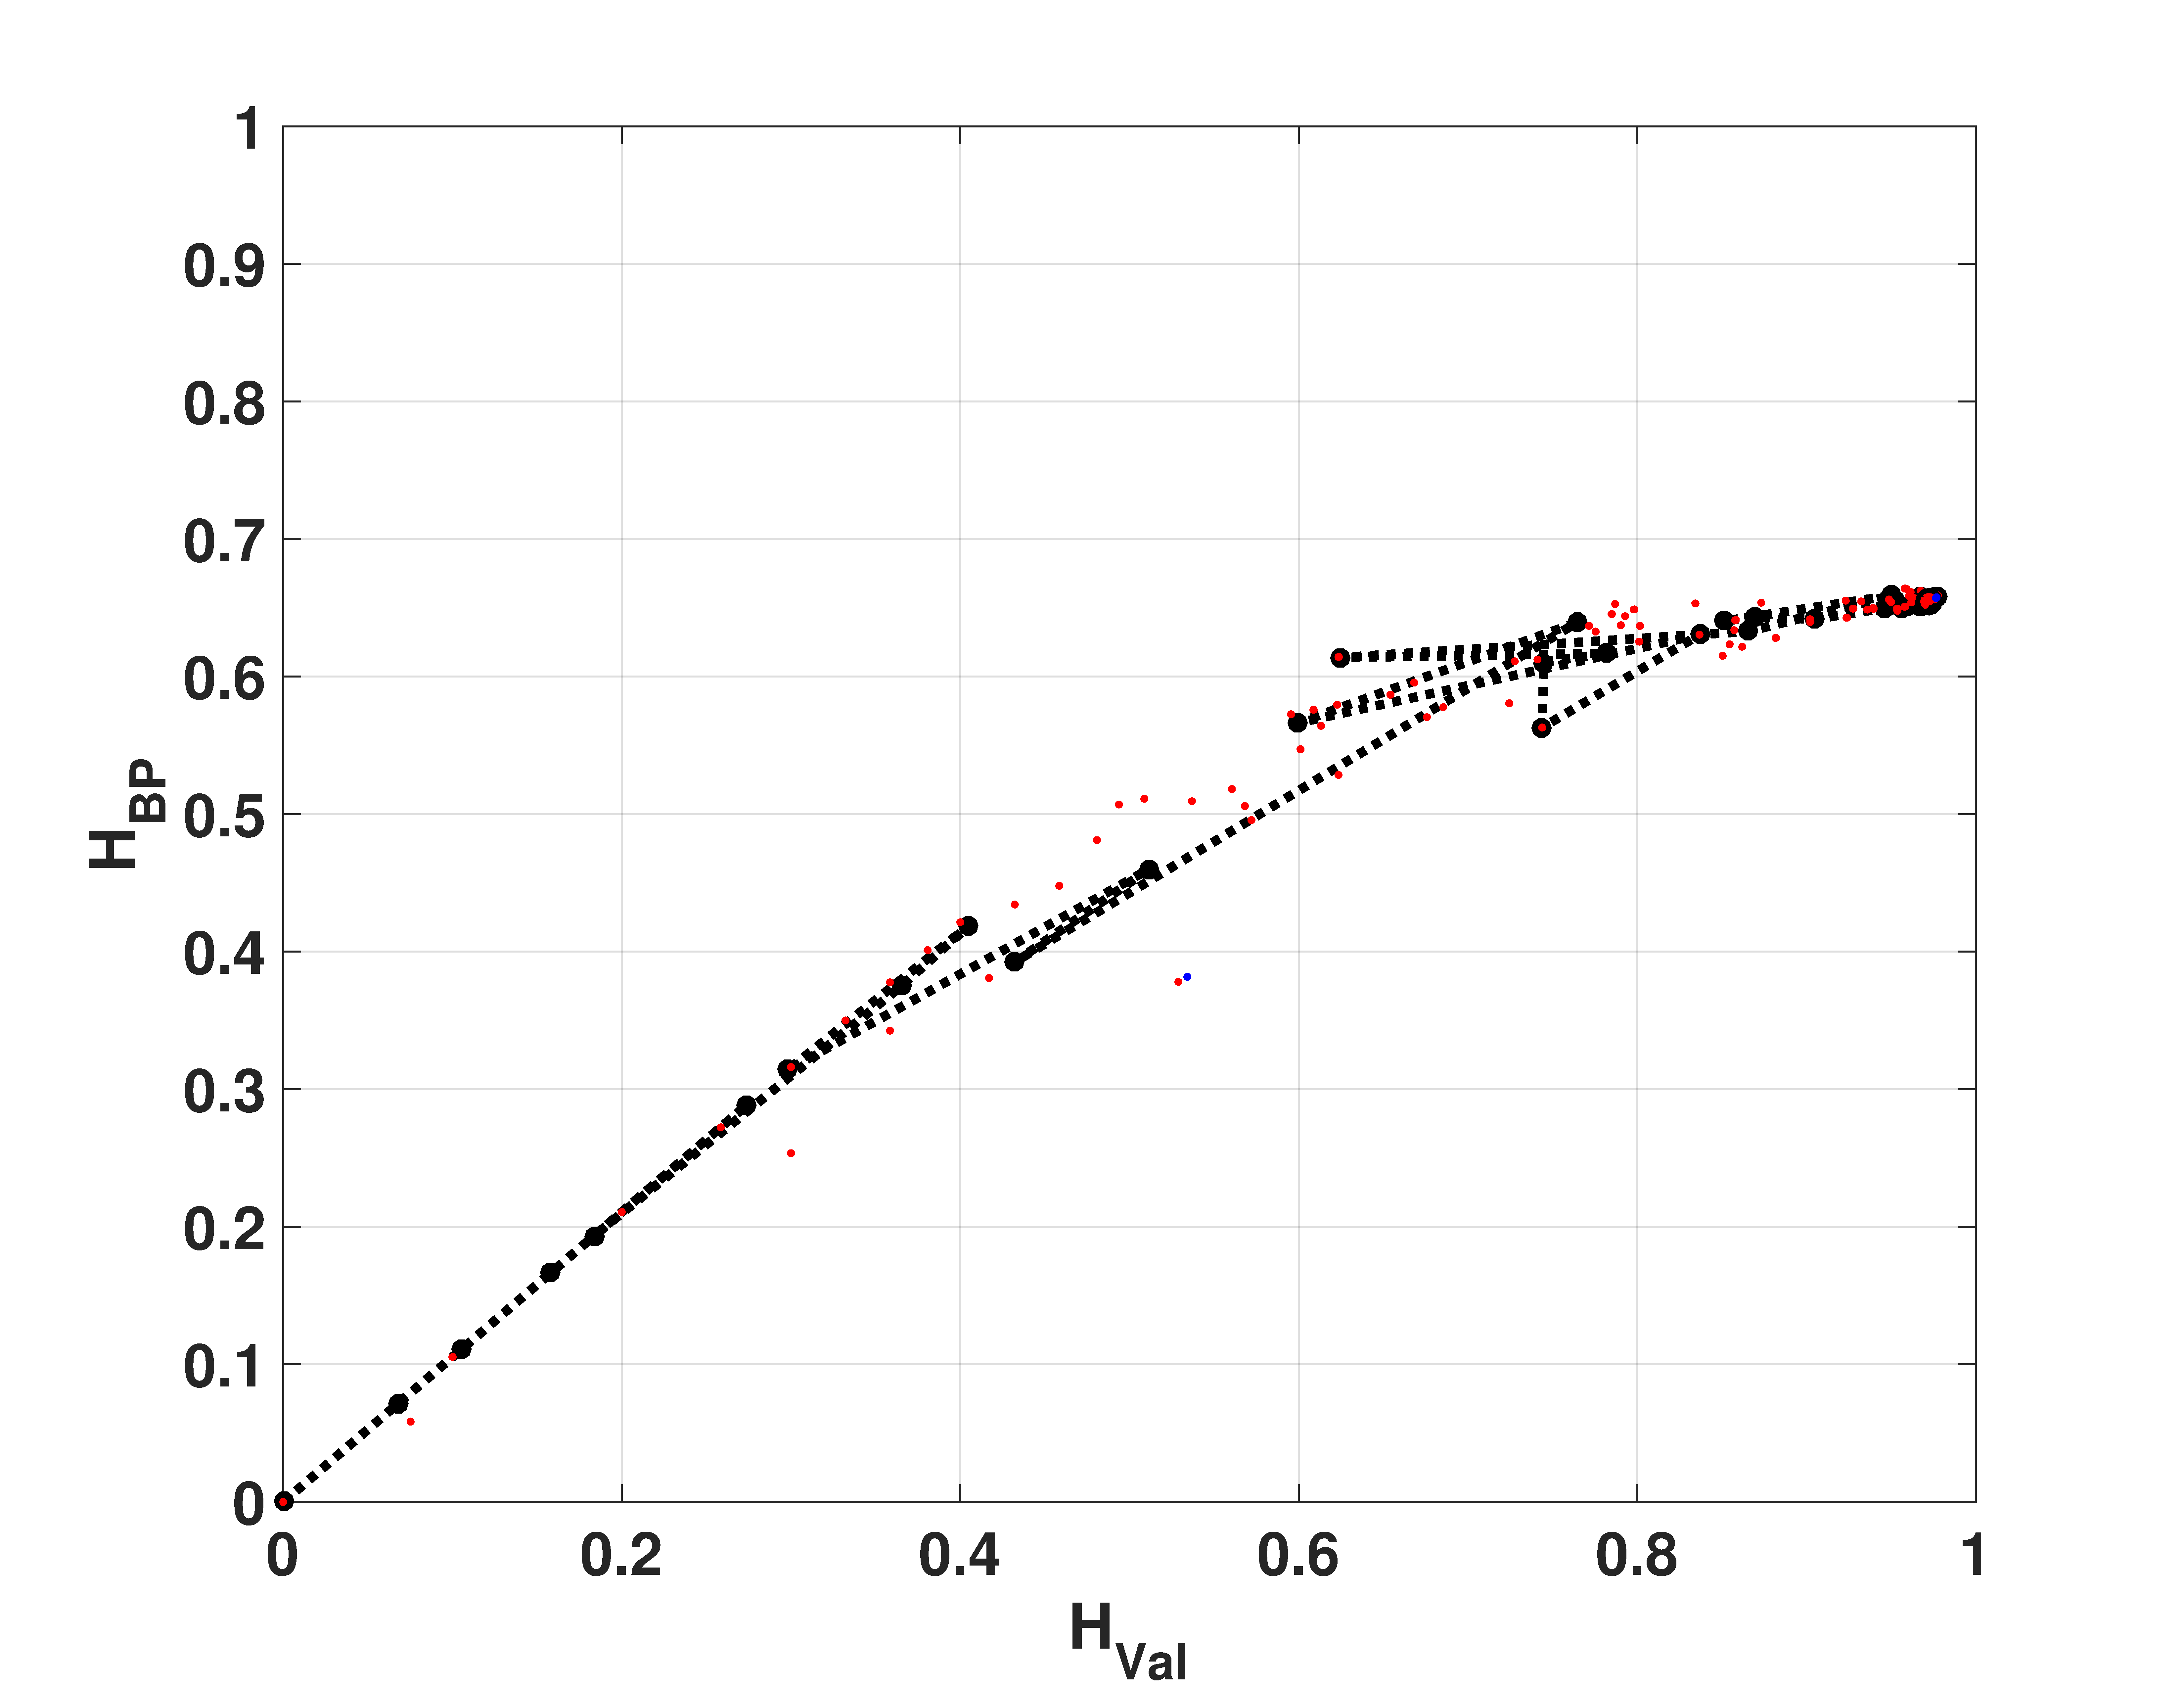
\includegraphics[width=.49\textwidth]{HbpHval_Switch}
	\caption{Evolution of statistical properties in double entropy plane of SWITCH map using binary representation: (a) $H_{val}$ vs $H_{BP}$ (b) $H_{val}$ vs $H_{BPW}$.}
	\label{fig:SWITCH_HH}
\end{figure}

Entropy complexity plane $C_{BP}$ vs $H_{BP}$ is showed in Fig. \ref{fig:SWITCH_HC}.
When we compare with the convergent point of LOG in this plane we can see that $C_{BP}$ is lower for SWITCH, this behaviour is more similar to an random generator.

\begin{figure}
	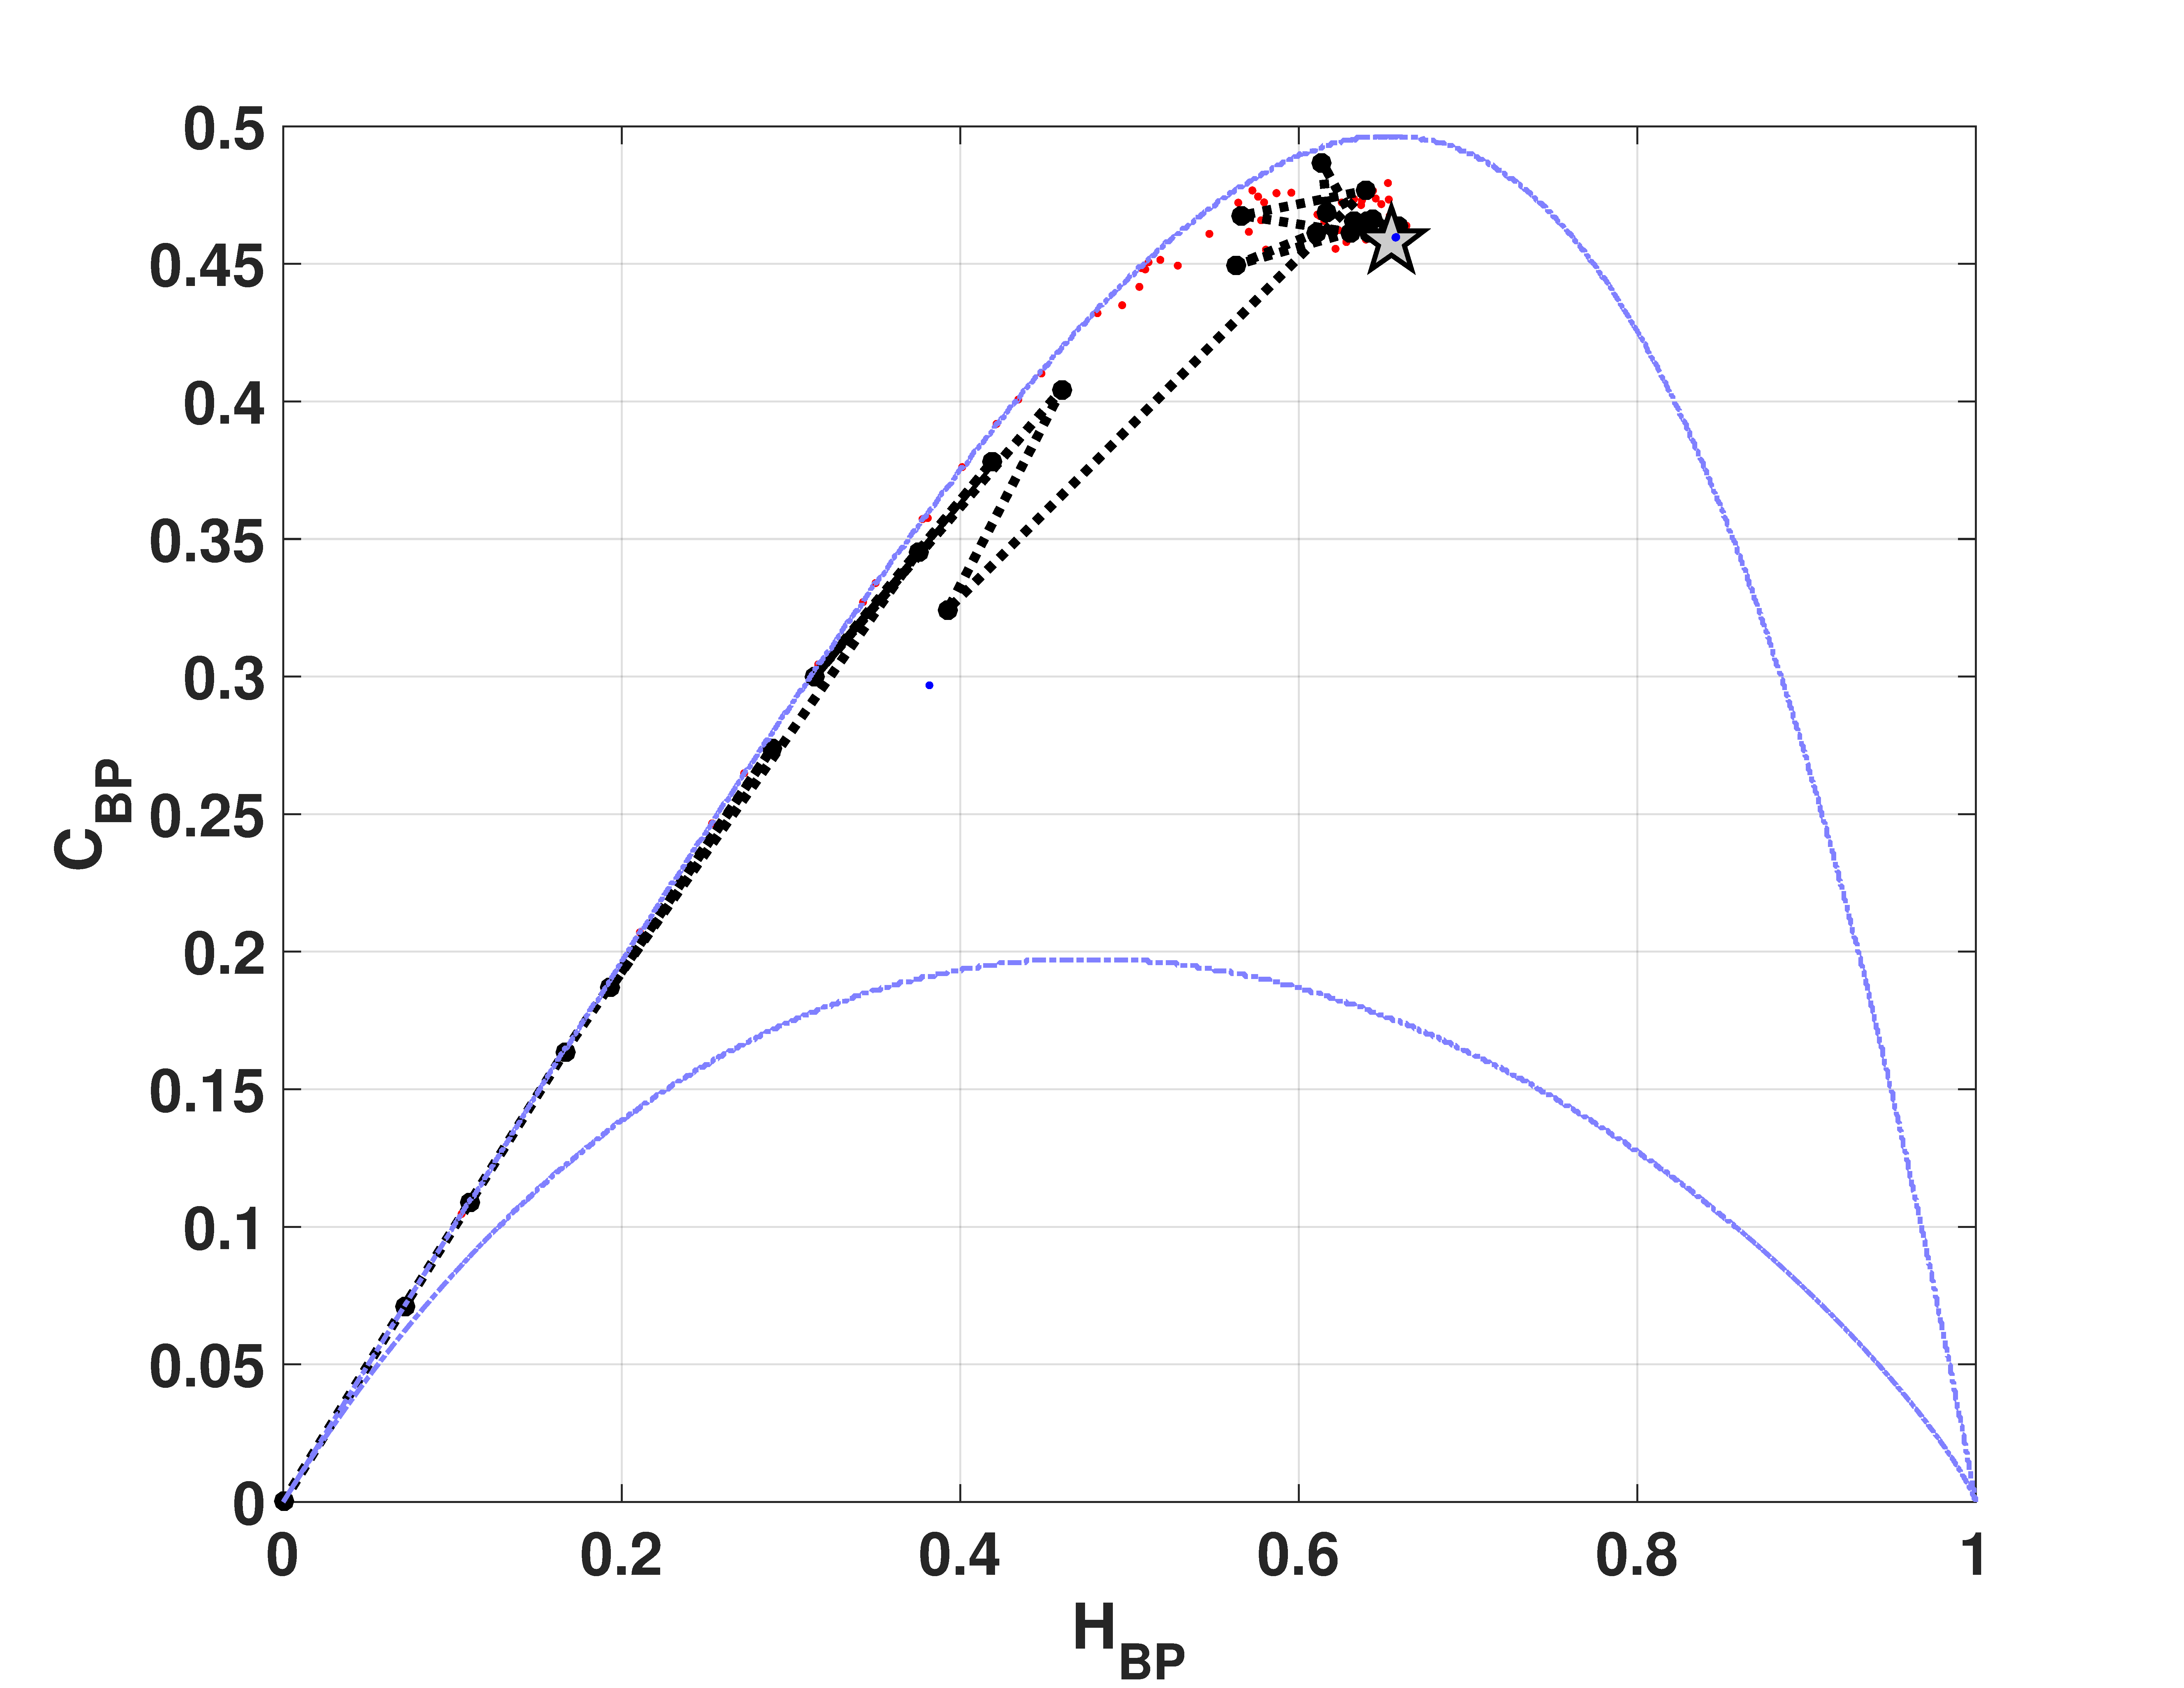
\includegraphics[width=.49\textwidth]{CbpHbp_Switch}
	\caption{Evolution of statistical properties in entropy-complexity plane of SWITCH map using binary representation: (a) $C_{BP}$ vs $H_{BP}$.}
	\label{fig:SWITCH_HC}
\end{figure}